\chapter{RESULTS AND DISCUSSION}

\section{Evidence Classification}
The results are classified by pathway and test condition before interpretation. A receiver CSV row, a mock stream, a simulator diagnostic, and a physical sensor trace have different evidential meaning. Table~\ref{tab:evidence-classification} prevents a successful bounded test from being presented as a broader system claim.

\begin{table}[H]
\centering
\small
\caption{Evidence classification used for reported observations.}
\label{tab:evidence-classification}
\begin{tabularx}{\textwidth}{p{39mm}p{45mm}Y}
\toprule
\textbf{Evidence} & \textbf{What it establishes} & \textbf{What it does not establish}\\
\midrule
Huawei relay receiver row & A relay payload reached and was stored by the authenticated local receiver. & Browser display of every row; clinical validity; direct Huawei API use.\\
Dashboard mock CSV & A synthetic stream was processed under its recorded run condition. & Live wearable throughput or clinical telemetry performance.\\
BLE mock counter & Mock routing handled the stated message count. & Device-specific BLE pairing or Huawei Band transport.\\
FreeRTOS host diagnostics & Behaviour of the Windows-hosted control runtime. & Hard real-time guarantee or genuine physiology.\\
Wokwi sketch & Simulated hardware/control logic and planned pin pathway. & Physical sensor acquisition or calibration.\\
\bottomrule
\end{tabularx}
\end{table}

\section{Genuine Wearable-Path Observation}
The receiver log contains Huawei-Health relay entries dated 22 October 2026. One complete record stores heart rate 60 BPM, SpO\textsubscript{2} 100\%, stress 57, and 4,181 steps, identified as \code{huawei\_band\_6\_healthapp}, \code{simulated=false}, and transport \code{health\_app\_ui}. The same record classifies heart rate and stress as real-time while labelling SpO\textsubscript{2} historical. A nearby earlier record stores 74 BPM, 100\% SpO\textsubscript{2}, stress 57, and 4,181 steps. These are documented relay observations, not clinical measurements.

\begin{table}[H]
\centering
\small
\caption{Selected documented Huawei-Health relay observations at the local receiver.}
\label{tab:genuine-observations}
\begin{tabularx}{\textwidth}{p{28mm}p{18mm}p{18mm}p{17mm}p{18mm}Y}
\toprule
\textbf{Receiver time} & \textbf{HR} & \textbf{SpO\textsubscript{2}} & \textbf{Stress} & \textbf{Steps} & \textbf{Qualification}\\
\midrule
2026-10-22 13:14:35 & 74 BPM & 100\% & 57 & 4,181 & Complete relay record; health-app UI transport.\\
2026-10-22 13:17:37 & 60 BPM & 100\% & 57 & 4,181 & HR/stress marked real-time; SpO\textsubscript{2} marked historical in the stored relay metadata.\\
2026-10-23 01:58 & 78 BPM & 99\% & absent & 5,432 & Later complete HR/SpO\textsubscript{2}/steps record; stress absent.\\
\bottomrule
\end{tabularx}
\end{table}

The bridge accepts only fresh, complete HR, SpO\textsubscript{2}, and steps according to its own contract. Because stress is not a shared schema field, the recorded stress observation cannot be claimed as mirror context. The inspected materials establish receiver-side acceptance and bridge eligibility logic; they do not contain a corresponding browser capture proving that every selected row reached the mirror. The genuine result is therefore qualified as \pmark.

\section{Schema and Bridge Validation}
Integration logic covers complete live snapshots, missing HR/SpO\textsubscript{2}/steps, stale values, simulated origin, and out-of-range values. The expected acceptance mapping for a valid live snapshot includes HR 74, SpO\textsubscript{2} 100, and steps 4,181 with activity \code{unknown}, motion intensity zero, \code{good} PPG quality proxy, and heuristic exertion. The negative paths demonstrate an important safety property: malformed or ineligible genuine-lane input is blocked before it becomes an apparently current dashboard value.

No statistic for live rejection rate is reported because a controlled representative sample count and test log for that rate were not identified. The result establishes branch behaviour in the available integration test and source, not a field reliability percentage.

\section{Dashboard Mock Stream}
The recorded dashboard session \code{session\_20261014\_193826.csv} contains 75 telemetry frames over 15 seconds with zero dropped frames in the associated documented mock run. Figure~\ref{fig:mock-telemetry} retains the source chart's explicit synthetic label. The chart consists of a mock sensor stream, so its apparent time trends must not be interpreted as genuine wearable biometrics.

\begin{figure}[H]
\centering
\begin{subfigure}[t]{0.48\textwidth}
  \centering
  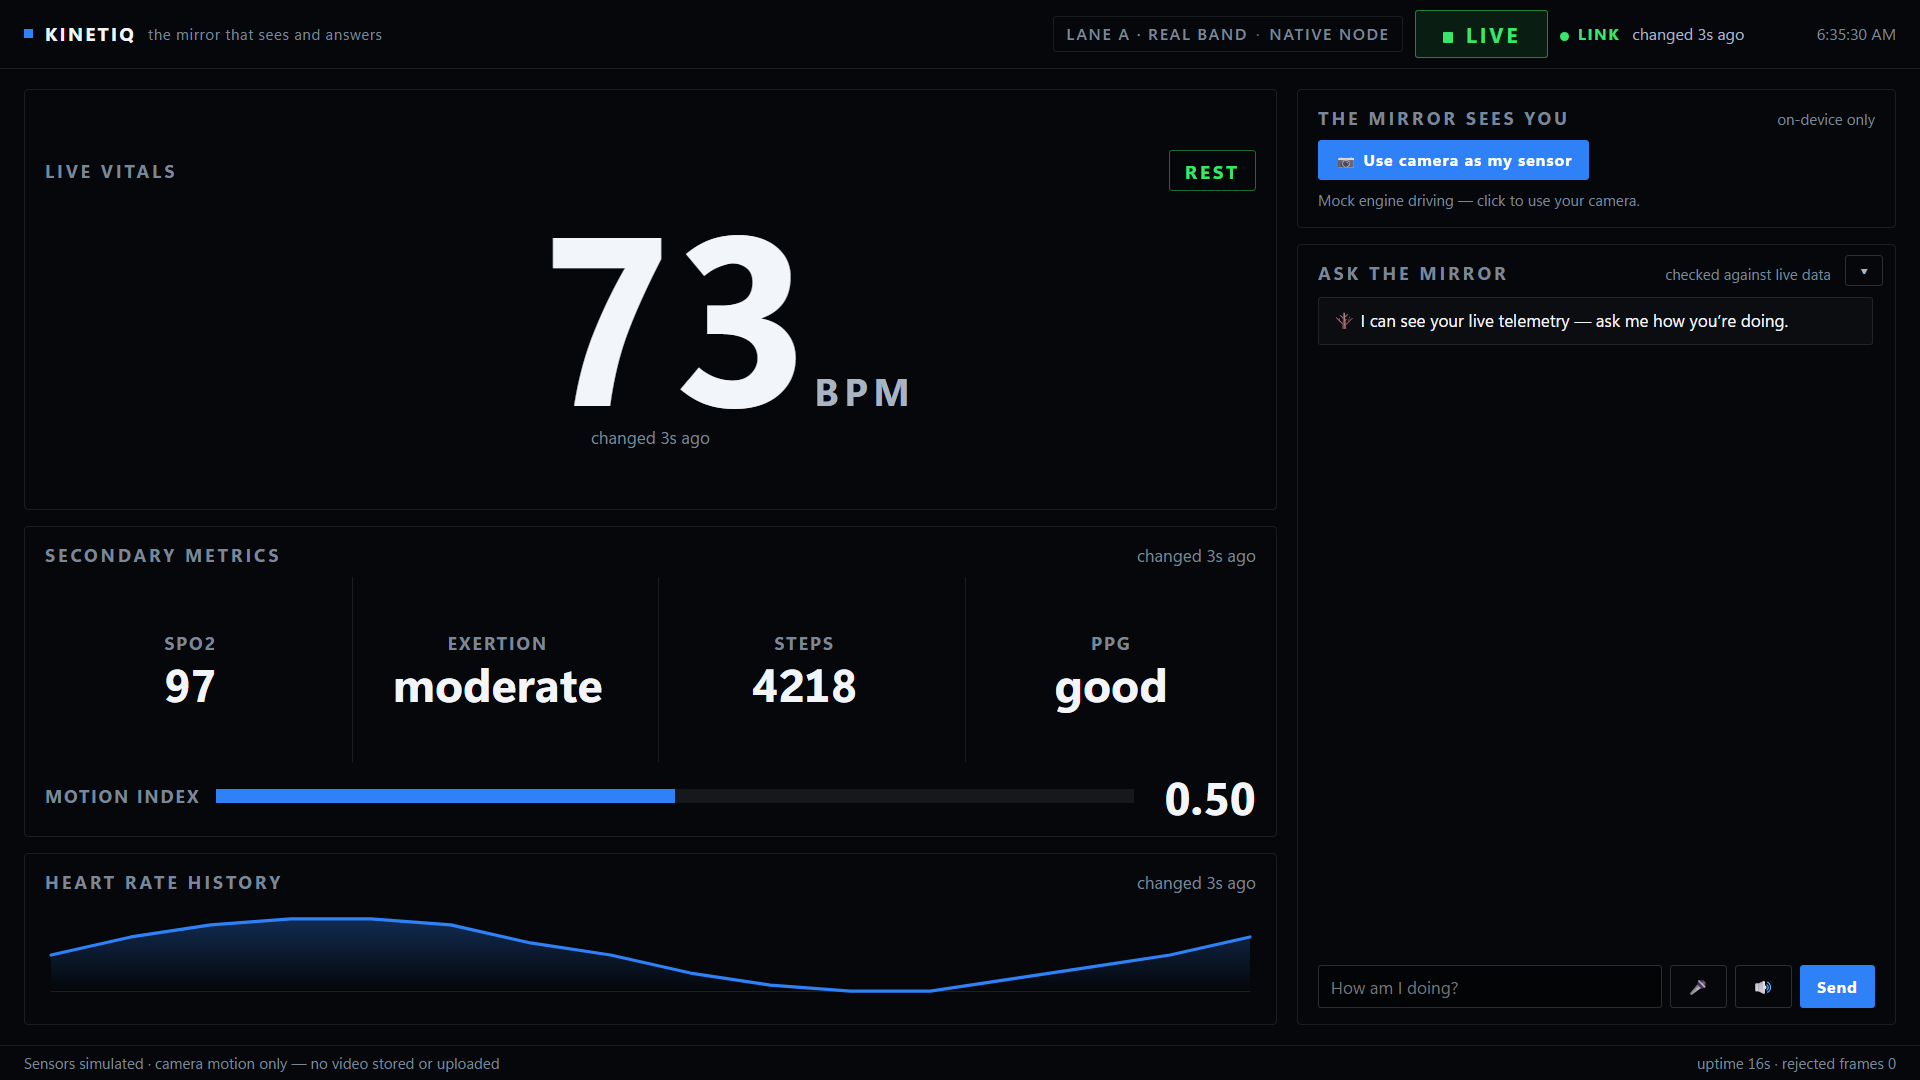
\includegraphics[width=\textwidth]{ui_live.png}
  \caption{Live}
  \label{fig:dashboard-states-live}
\end{subfigure}\hfill
\begin{subfigure}[t]{0.48\textwidth}
  \centering
  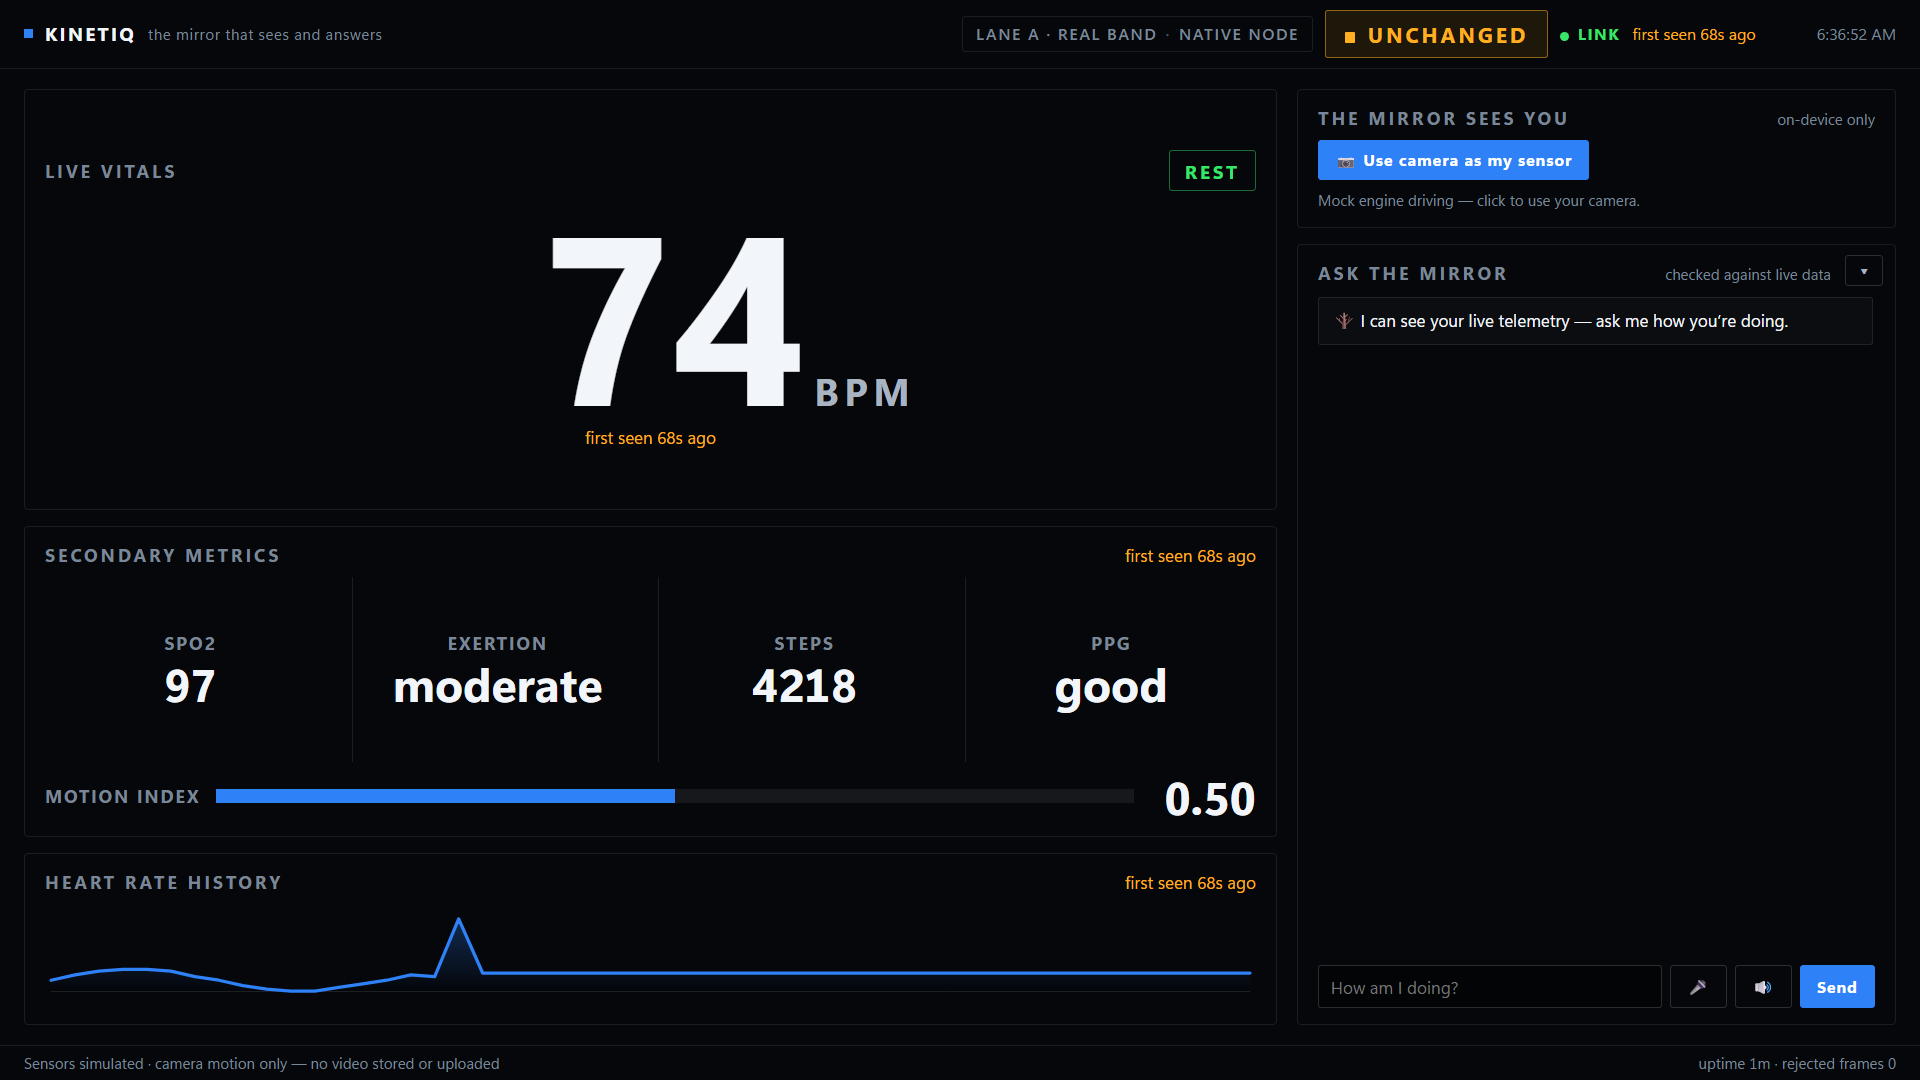
\includegraphics[width=\textwidth]{ui_unchanged.png}
  \caption{Unchanged}
  \label{fig:dashboard-states-unchanged}
\end{subfigure}\\[3pt]
\begin{subfigure}[t]{0.48\textwidth}
  \centering
  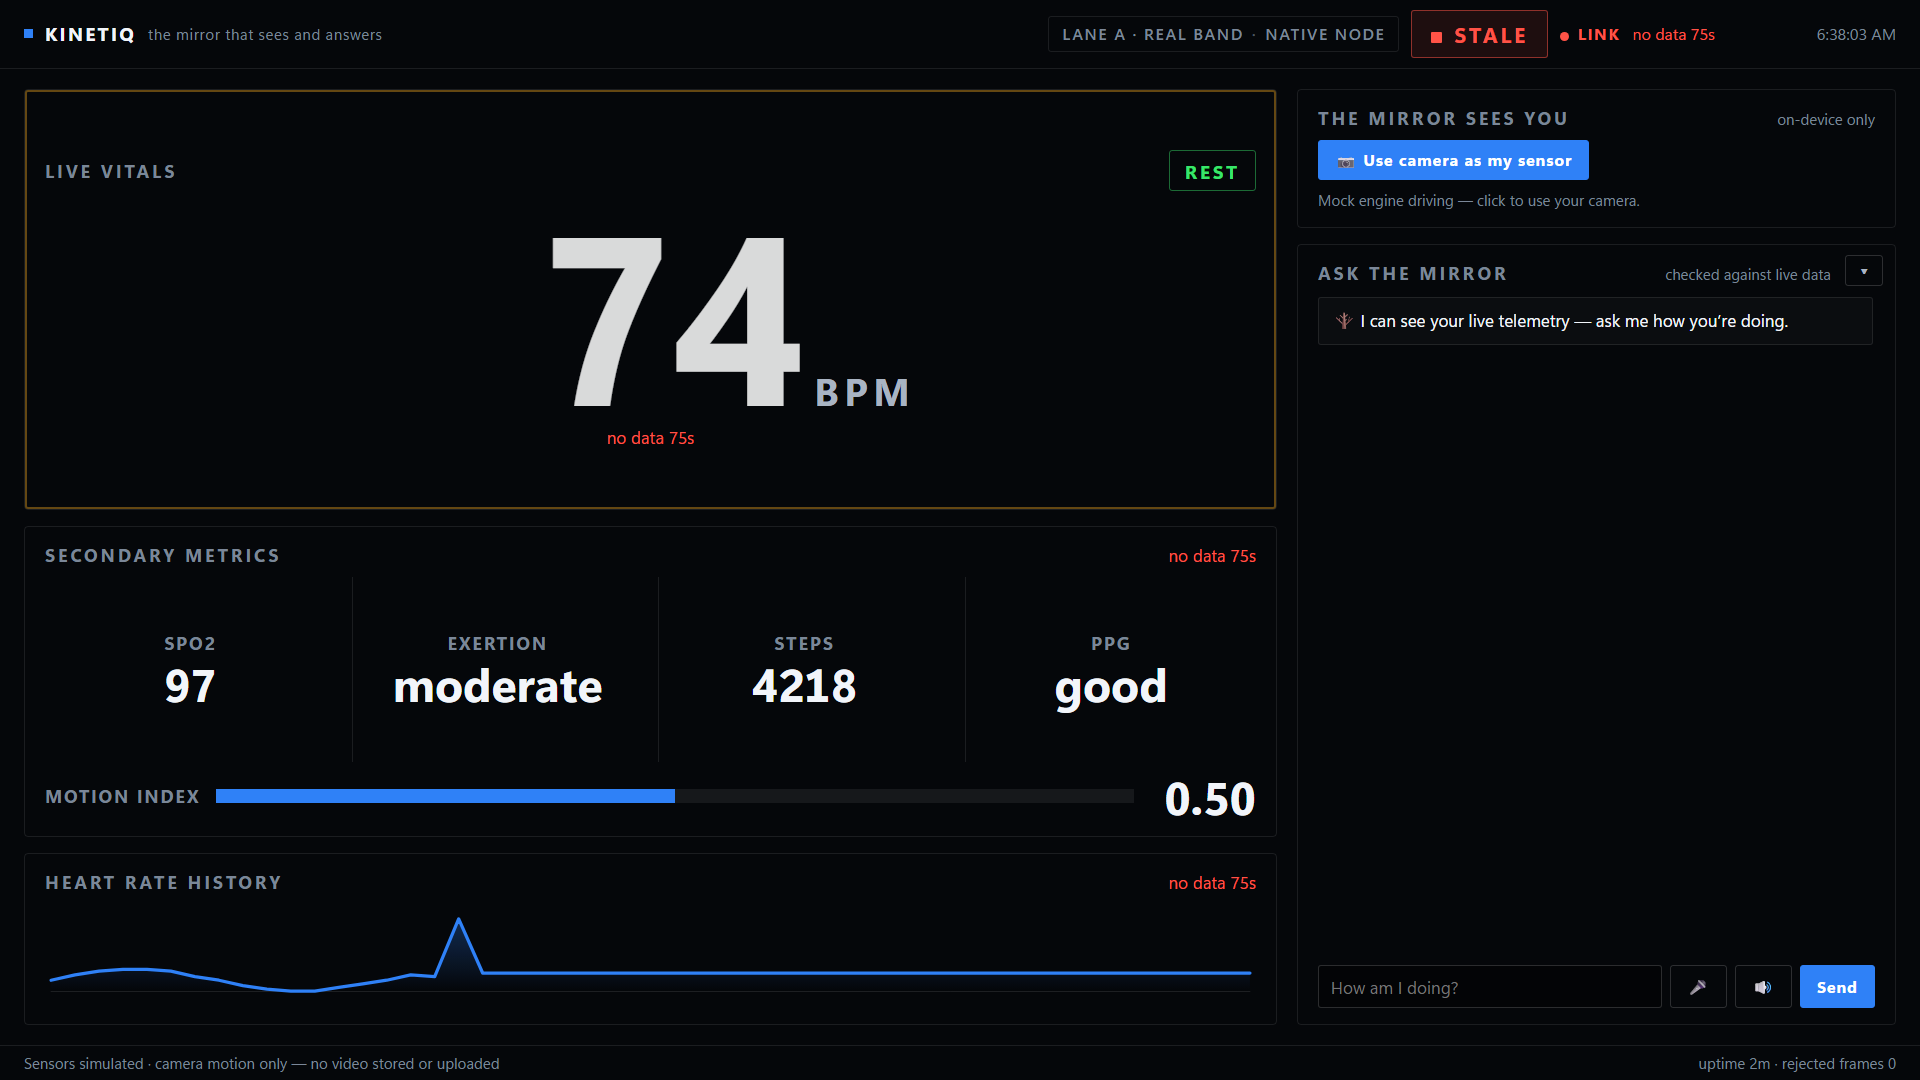
\includegraphics[width=\textwidth]{ui_stale.png}
  \caption{Stale}
  \label{fig:dashboard-states-stale}
\end{subfigure}\hfill
\begin{subfigure}[t]{0.48\textwidth}
  \centering
  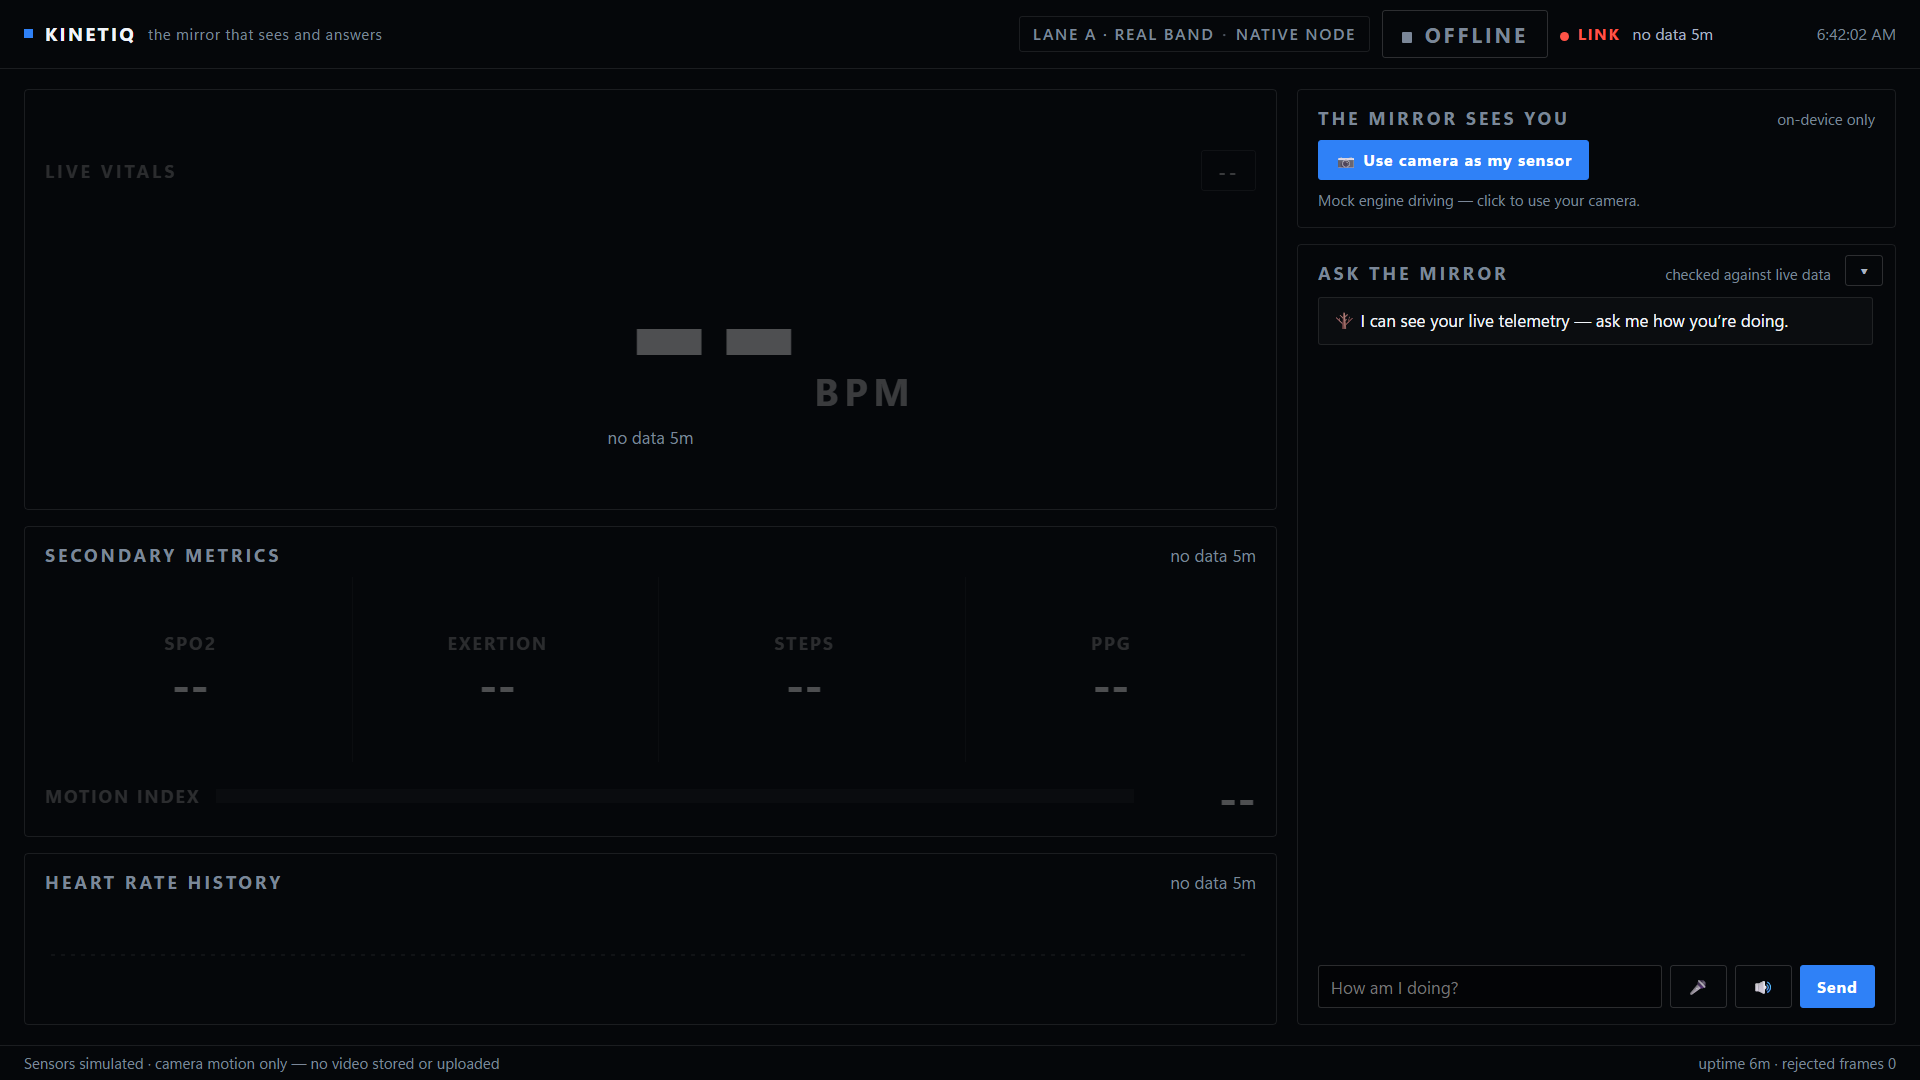
\includegraphics[width=\textwidth]{ui_offline.png}
  \caption{Offline}
  \label{fig:dashboard-states-offline}
\end{subfigure}
\caption[Dashboard freshness states (synthetic input)]{Dashboard freshness states observed under controlled synthetic input: live, unchanged, stale and offline. These captures exercise the freshness/offline logic; they are not live wearable telemetry.}
\label{fig:dashboard-states}
\end{figure}

\begin{figure}[H]
\centering
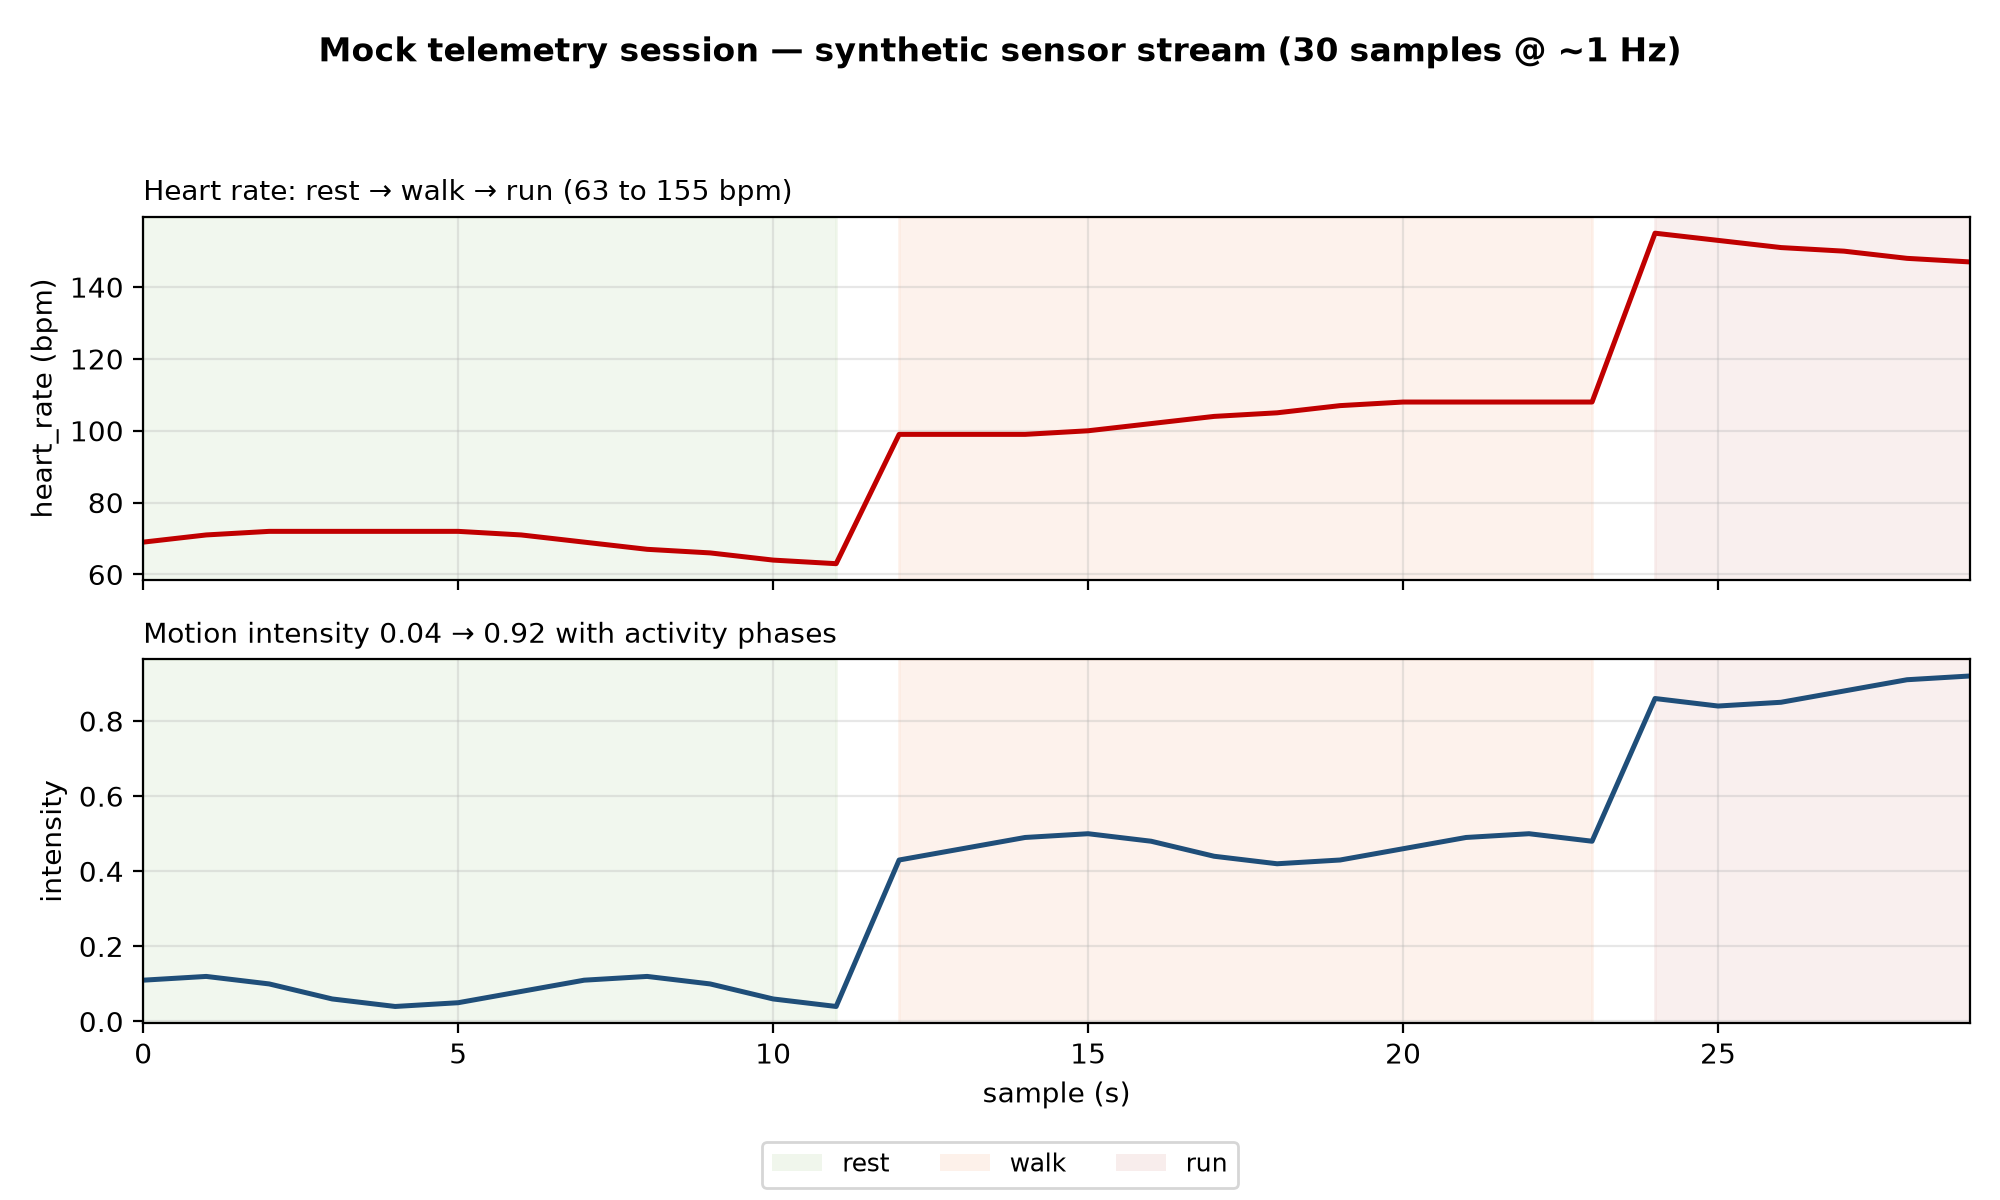
\includegraphics[width=\textwidth]{mock_telemetry_results.png}
\caption[Mock telemetry session (synthetic, 30 samples)]{Mock telemetry session: synthetic sensor stream (30 samples at approximately 1 Hz) from the project materials. It is not a genuine biometric time series.}
\label{fig:mock-telemetry}
\end{figure}

The zero-drop result establishes that the documented mock dashboard session maintained its recorded frame count under those input and host conditions. It does not establish throughput for the phone relay, an arbitrary browser load, or all live wearable sessions.

\section{BLE Mock and Voice Observation}
The BLE client mock is configured with \code{--source mock --mock-count 30}; the project result records 30 routed messages with zero rejections. This confirms the mock route and its message handling for the defined input. It does not confirm physical BLE communication with Huawei Band 6 or any other wearable.

The voice pipeline result records 0.48 s for faster-whisper transcription of a synthesized audio clip. The software uses the \code{tiny.en} model with \code{int8} inference. The metric is useful for a local demonstration latency budget, but it does not assess live microphone capture, noise, language variation, or correctness of a wellness utterance.

\section{RTOS Control and Offline Fallback}
The native control node exposes period, lateness, queue high-water mark, dropped events, and missed-deadline fields while generating contract-compatible synthetic telemetry. Rest, walk, run, fall, and automatic controls are mapped through the console. The single-writer design and diagnostic fields make the fallback observable and reduce ambiguity during a demonstration. The host execution remains a Windows simulator, so the results support source-level task design and runtime diagnostics rather than a hard-deadline assertion.

When genuine transport cannot provide a complete live snapshot, the RTOS route supports a repeatable interface demonstration. It must be labelled as control or simulated data in the dashboard and narration. Treating the synthetic lane as a physiological backup would defeat the provenance boundary that the design is intended to protect.

\section{Grounding Verdict Behaviour}
The assistant renders a grounding verdict after comparing response text with accepted telemetry. A \texttt{PASS} denotes agreement under the implemented keyword/value checks. A \texttt{FAIL} identifies a mismatch in those checks. Neither observation validates medical content. The available code continues text-to-speech after the verdict, including a failure, so a \texttt{FAIL} is a visible warning rather than a suppression mechanism. Further work should make output gating and test fixtures explicit if fail-closed behaviour is required.

\section{Hardware and Budget Reconciliation}
The physical embedded hardware remains planned or simulated. The final-review component table lists INR~998 for two ESP32 boards, INR~470 for the MPU6050/HC-SR04/IR group, and INR~808 for DHT22 plus breadboard/jumper support. Those listed subtotals sum to INR~2,276. The same source also contains an approximate INR~1,950 Tier-A statement, which is not supported by the displayed component amounts. Table~\ref{tab:bom-reconciliation} retains the reproducible subtotal and excludes the inconsistent figure from any verified budget claim.

\begin{table}[H]
\centering
\small
\caption{Reconciled component subtotal from the displayed final-review BOM.}
\label{tab:bom-reconciliation}
\begin{tabularx}{\textwidth}{Yp{32mm}p{37mm}}
\toprule
\textbf{Displayed category} & \textbf{Amount} & \textbf{Interpretation}\\
\midrule
Two ESP32 development boards & INR~998 & Listed category subtotal.\\
MPU6050, HC-SR04, and IR group & INR~470 & Listed category subtotal.\\
DHT22, breadboard, and jumper group & INR~808 & Listed category subtotal.\\
\midrule
\textbf{Recalculated displayed subtotal} & \textbf{INR~2,276} & 998 + 470 + 808.\\
Earlier Tier-A statement & INR~1,950 & Not retained as verified: its revision/itemisation is not recoverable from the displayed table.\\
\bottomrule
\end{tabularx}
\end{table}

\section{Overall Verification Summary}
The strongest verified elements are the eight-field validation logic, dashboard freshness design, native FreeRTOS task structure, synthetic fallback, and documented local receiver records. The genuine wearable path is partially demonstrated through relay data and bridge rules but lacks complete browser-render evidence for each cited observation. Voice and grounding modules are implemented but only receive narrow test evidence. Physical sensors remain outside the validated final runtime. These qualifications preserve the engineering value of the working modules without extending the evidence beyond its scope.
